\documentclass[12pt]{article}

\usepackage{tikz}
\usetikzlibrary{calc}
\usepackage{pgfplots}
\usepackage{longtable}
\usepackage{hyperref}
\usepackage{enumitem}
\usepackage[nocenter]{qtree}
\usepackage{tree-dvips}
\usepackage{amsmath}

\renewcommand\thesection{\large\underline{Problem \arabic{section}}}

\title{\vspace{-3em}\underline{CS 440: Assignment 1}}
\author{
  Ian Manske (im302) section 2\\
  Mateusz Chojnowski (mc2106) section 2\\
  Kenneth Quizon (kbq6) section 3}
\date{October 19, 2022}

\begin{document}

\maketitle

\section{}
\begin{enumerate}[label={\large\textbf{\alph*)}}]
\item
Our visualization is able to show:
\begin{itemize}
  \item the min cost path found by the search algorithm (red)
  \item the vertices in the closed list (yellow)
  \item the vertices in the open list (cyan)
  \item the start and goal vertex (green and blue respectively)
  \item the parents of all verticies that have a parent (indicated by a colored line)
  \item blocked cells (the gray filled cells)
  \item the current vertex at the current iteration of the search algorithm (magenta)
\end{itemize}

This is all done by painting a canvas. Because the canvas can be zoomed in and out
via buttons on the right, it was placed within a scroll-pane.

Naturally, the $f$, $g$, and $h$ values for a specific vertex are also displayed on the right.
Two textfields for the $x$ and $y$ coordinate can be edited to view the values for any vertex.
For greater convenience and debugging potential, our visualization also has a ``step'' capability.
Clicking the ``Step'' button advances the search algorithm by one iteration / vertex.
This automatically displays the $f$, $g$, and $h$ values for the new current vertex as well.
The ``Run'' button, on the other hand, runs the algorithm to completion.
Otherwise, one can also switch between A* and Theta* on the GUI,
and a reset button is provided to clear the current search.
The grid file is specified through the command line,
and a random $100 \times 50$ grid is generated if none is provided.
See the \verb|README.md| for more information regarding the CLI.

\item Trace of A*

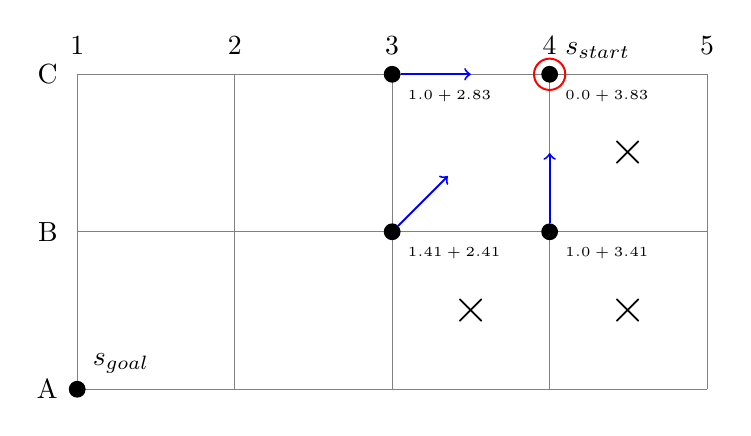
\begin{tikzpicture}[scale=2.0]
\draw [step=1.cm, color=gray] (0, 0) grid (4, 2);
\node [label=left:{C}] at (0, 2) {};
\node [label=left:{B}] at (0, 1) {};
\node [label=left:{A}] at (0, 0) {};
\node [label=above:{1}] at (0, 2) {};
\node [label=above:{2}] at (1, 2) {};
\node [label=above:{3}] at (2, 2) {};
\node [label=above:{4}] at (3, 2) {};
\node [label=above:{5}] at (4, 2) {};

\node at (3.5, 1.5) {\LARGE $\times$};
\node at (2.5, 0.5) {\LARGE $\times$};
\node at (3.5, 0.5) {\LARGE $\times$};

\node [label=above right:{$s_{start}$}, label=below right:{\tiny$0.0 + 3.83$}, draw, circle, fill, inner sep=2pt] (start) at (3, 2) {};
\node [label=above right:{$s_{goal}$}, draw, circle, fill, inner sep=2pt] at (0, 0) {};

\node [draw, circle, color=red, line width=0.25mm, inner sep=4pt] at (start) {};

\node [label=below right:{\tiny$1.0 + 2.83$}, draw, circle, fill, inner sep=2pt] (C3) at (2, 2) {};
\node [label=below right:{\tiny$1.41 + 2.41$}, draw, circle, fill, inner sep=2pt] (B3) at (2, 1) {};
\node [label=below right:{\tiny$1.0 + 3.41$}, draw, circle, fill, inner sep=2pt] (B4) at (3, 1) {};
\draw [->, line width=0.25mm, blue] (C3) -- ($(C3)!0.5cm!(start)$);
\draw [->, line width=0.25mm, blue] (B3) -- ($(B3)!0.5cm!(start)$);
\draw [->, line width=0.25mm, blue] (B4) -- ($(B4)!0.5cm!(start)$);
\end{tikzpicture}

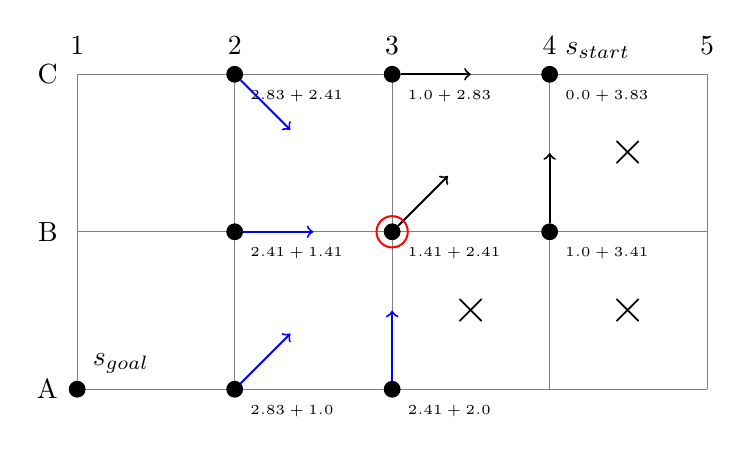
\begin{tikzpicture}[scale=2.0]
\draw [step=1.cm, color=gray] (0, 0) grid (4, 2);
\node [label=left:{C}] at (0, 2) {};
\node [label=left:{B}] at (0, 1) {};
\node [label=left:{A}] at (0, 0) {};
\node [label=above:{1}] at (0, 2) {};
\node [label=above:{2}] at (1, 2) {};
\node [label=above:{3}] at (2, 2) {};
\node [label=above:{4}] at (3, 2) {};
\node [label=above:{5}] at (4, 2) {};

\node at (3.5, 1.5) {\LARGE $\times$};
\node at (2.5, 0.5) {\LARGE $\times$};
\node at (3.5, 0.5) {\LARGE $\times$};

\node [label=above right:{$s_{start}$}, label=below right:{\tiny$0.0 + 3.83$}, draw, circle, fill, inner sep=2pt] (start) at (3, 2) {};
\node [label=above right:{$s_{goal}$}, draw, circle, fill, inner sep=2pt] at (0, 0) {};

\node [label=below right:{\tiny$1.0 + 2.83$}, draw, circle, fill, inner sep=2pt] (C3) at (2, 2) {};
\node [label=below right:{\tiny$1.41 + 2.41$}, draw, circle, fill, inner sep=2pt] (B3) at (2, 1) {};
\node [label=below right:{\tiny$1.0 + 3.41$}, draw, circle, fill, inner sep=2pt] (B4) at (3, 1) {};
\draw [->, line width=0.25mm, black] (C3) -- ($(C3)!0.5cm!(start)$);
\draw [->, line width=0.25mm, black] (B3) -- ($(B3)!0.5cm!(start)$);
\draw [->, line width=0.25mm, black] (B4) -- ($(B4)!0.5cm!(start)$);

\node [draw, circle, color=red, line width=0.25mm, inner sep=4pt] at (B3) {};

\node [label=below right:{\tiny$2.41 + 2.0$}, draw, circle, fill, inner sep=2pt] (A3) at (2, 0) {};
\node [label=below right:{\tiny$2.83 + 2.41$}, draw, circle, fill, inner sep=2pt] (C2) at (1, 2) {};
\node [label=below right:{\tiny$2.41 + 1.41$}, draw, circle, fill, inner sep=2pt] (B2) at (1, 1) {};
\node [label=below right:{\tiny$2.83 + 1.0$}, draw, circle, fill, inner sep=2pt] (A2) at (1, 0) {};
\draw [->, line width=0.25mm, blue] (A3) -- ($(A3)!0.5cm!(B3)$);
\draw [->, line width=0.25mm, blue] (C2) -- ($(C2)!0.5cm!(B3)$);
\draw [->, line width=0.25mm, blue] (B2) -- ($(B2)!0.5cm!(B3)$);
\draw [->, line width=0.25mm, blue] (A2) -- ($(A2)!0.5cm!(B3)$);
\end{tikzpicture}

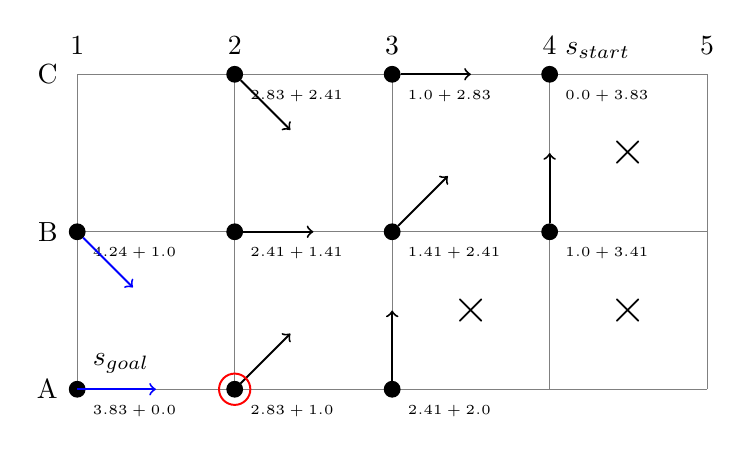
\begin{tikzpicture}[scale=2.0]
\draw [step=1.cm, color=gray] (0, 0) grid (4, 2);
\node [label=left:{C}] at (0, 2) {};
\node [label=left:{B}] at (0, 1) {};
\node [label=left:{A}] at (0, 0) {};
\node [label=above:{1}] at (0, 2) {};
\node [label=above:{2}] at (1, 2) {};
\node [label=above:{3}] at (2, 2) {};
\node [label=above:{4}] at (3, 2) {};
\node [label=above:{5}] at (4, 2) {};

\node at (3.5, 1.5) {\LARGE $\times$};
\node at (2.5, 0.5) {\LARGE $\times$};
\node at (3.5, 0.5) {\LARGE $\times$};

\node [label=above right:{$s_{start}$}, label=below right:{\tiny$0.0 + 3.83$}, draw, circle, fill, inner sep=2pt] (start) at (3, 2) {};
\node [label=above right:{$s_{goal}$}, label=below right:{\tiny$3.83 + 0.0$}, draw, circle, fill, inner sep=2pt] at (0, 0) {};

\node [label=below right:{\tiny$1.0 + 2.83$}, draw, circle, fill, inner sep=2pt] (C3) at (2, 2) {};
\node [label=below right:{\tiny$1.41 + 2.41$}, draw, circle, fill, inner sep=2pt] (B3) at (2, 1) {};
\node [label=below right:{\tiny$1.0 + 3.41$}, draw, circle, fill, inner sep=2pt] (B4) at (3, 1) {};
\draw [->, line width=0.25mm, black] (C3) -- ($(C3)!0.5cm!(start)$);
\draw [->, line width=0.25mm, black] (B3) -- ($(B3)!0.5cm!(start)$);
\draw [->, line width=0.25mm, black] (B4) -- ($(B4)!0.5cm!(start)$);

\node [label=below right:{\tiny$2.41 + 2.0$}, draw, circle, fill, inner sep=2pt] (A3) at (2, 0) {};
\node [label=below right:{\tiny$2.83 + 2.41$}, draw, circle, fill, inner sep=2pt] (C2) at (1, 2) {};
\node [label=below right:{\tiny$2.41 + 1.41$}, draw, circle, fill, inner sep=2pt] (B2) at (1, 1) {};
\node [label=below right:{\tiny$2.83 + 1.0$}, draw, circle, fill, inner sep=2pt] (A2) at (1, 0) {};
\draw [->, line width=0.25mm, black] (A3) -- ($(A3)!0.5cm!(B3)$);
\draw [->, line width=0.25mm, black] (C2) -- ($(C2)!0.5cm!(B3)$);
\draw [->, line width=0.25mm, black] (B2) -- ($(B2)!0.5cm!(B3)$);
\draw [->, line width=0.25mm, black] (A2) -- ($(A2)!0.5cm!(B3)$);

\node [draw, circle, color=red, line width=0.25mm, inner sep=4pt] at (A2) {};

\node [label=below right:{\tiny$4.24 + 1.0$}, draw, circle, fill, inner sep=2pt] (B1) at (0, 1) {};
\draw [->, line width=0.25mm, blue] (B1) -- ($(B1)!0.5cm!(A2)$);
\draw [->, line width=0.25mm, blue] (0, 0) -- ($(0, 0)!0.5cm!(A2)$);
\end{tikzpicture}

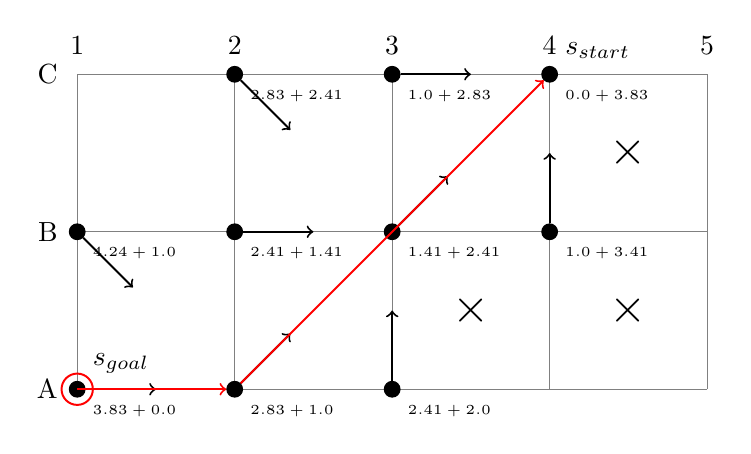
\begin{tikzpicture}[scale=2.0]
\draw [step=1.cm, color=gray] (0, 0) grid (4, 2);
\node [label=left:{C}] at (0, 2) {};
\node [label=left:{B}] at (0, 1) {};
\node [label=left:{A}] at (0, 0) {};
\node [label=above:{1}] at (0, 2) {};
\node [label=above:{2}] at (1, 2) {};
\node [label=above:{3}] at (2, 2) {};
\node [label=above:{4}] at (3, 2) {};
\node [label=above:{5}] at (4, 2) {};

\node at (3.5, 1.5) {\LARGE $\times$};
\node at (2.5, 0.5) {\LARGE $\times$};
\node at (3.5, 0.5) {\LARGE $\times$};

\node [label=above right:{$s_{start}$}, label=below right:{\tiny$0.0 + 3.83$}, draw, circle, fill, inner sep=2pt] (start) at (3, 2) {};
\node [label=above right:{$s_{goal}$}, label=below right:{\tiny$3.83 + 0.0$}, draw, circle, fill, inner sep=2pt] at (0, 0) {};

\node [label=below right:{\tiny$1.0 + 2.83$}, draw, circle, fill, inner sep=2pt] (C3) at (2, 2) {};
\node [label=below right:{\tiny$1.41 + 2.41$}, draw, circle, fill, inner sep=2pt] (B3) at (2, 1) {};
\node [label=below right:{\tiny$1.0 + 3.41$}, draw, circle, fill, inner sep=2pt] (B4) at (3, 1) {};
\draw [->, line width=0.25mm, black] (C3) -- ($(C3)!0.5cm!(start)$);
\draw [->, line width=0.25mm, black] (B3) -- ($(B3)!0.5cm!(start)$);
\draw [->, line width=0.25mm, black] (B4) -- ($(B4)!0.5cm!(start)$);

\node [label=below right:{\tiny$2.41 + 2.0$}, draw, circle, fill, inner sep=2pt] (A3) at (2, 0) {};
\node [label=below right:{\tiny$2.83 + 2.41$}, draw, circle, fill, inner sep=2pt] (C2) at (1, 2) {};
\node [label=below right:{\tiny$2.41 + 1.41$}, draw, circle, fill, inner sep=2pt] (B2) at (1, 1) {};
\node [label=below right:{\tiny$2.83 + 1.0$}, draw, circle, fill, inner sep=2pt] (A2) at (1, 0) {};
\draw [->, line width=0.25mm, black] (A3) -- ($(A3)!0.5cm!(B3)$);
\draw [->, line width=0.25mm, black] (C2) -- ($(C2)!0.5cm!(B3)$);
\draw [->, line width=0.25mm, black] (B2) -- ($(B2)!0.5cm!(B3)$);
\draw [->, line width=0.25mm, black] (A2) -- ($(A2)!0.5cm!(B3)$);

\node [label=below right:{\tiny$4.24 + 1.0$}, draw, circle, fill, inner sep=2pt] (B1) at (0, 1) {};
\draw [->, line width=0.25mm, black] (B1) -- ($(B1)!0.5cm!(A2)$);
\draw [->, line width=0.25mm, black] (0, 0) -- ($(0, 0)!0.5cm!(A2)$);

\node [draw, circle, color=red, line width=0.25mm, inner sep=4pt] at (0, 0) {};

\draw [->, line width=0.25mm, red] (A2) -- (start);
\draw [->, line width=0.25mm, red] (0, 0) -- (A2);
\end{tikzpicture}

Trace of Theta*

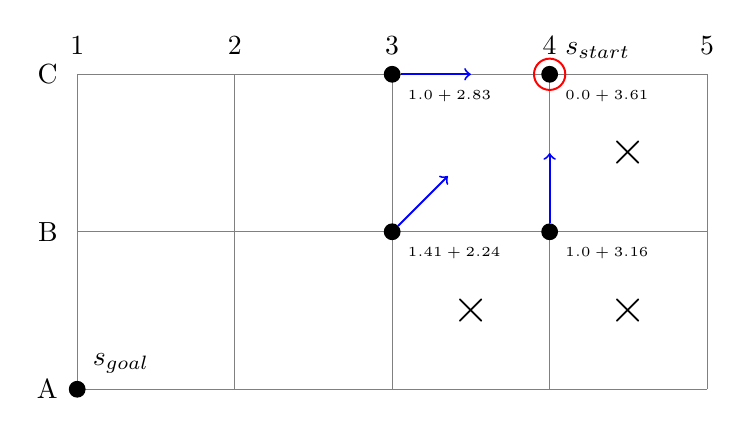
\begin{tikzpicture}[scale=2.0]
\draw [step=1.cm, color=gray] (0, 0) grid (4, 2);
\node [label=left:{C}] at (0, 2) {};
\node [label=left:{B}] at (0, 1) {};
\node [label=left:{A}] at (0, 0) {};
\node [label=above:{1}] at (0, 2) {};
\node [label=above:{2}] at (1, 2) {};
\node [label=above:{3}] at (2, 2) {};
\node [label=above:{4}] at (3, 2) {};
\node [label=above:{5}] at (4, 2) {};

\node at (3.5, 1.5) {\LARGE $\times$};
\node at (2.5, 0.5) {\LARGE $\times$};
\node at (3.5, 0.5) {\LARGE $\times$};

\node [label=above right:{$s_{start}$}, label=below right:{\tiny$0.0 + 3.61$}, draw, circle, fill, inner sep=2pt] (start) at (3, 2) {};
\node [label=above right:{$s_{goal}$}, draw, circle, fill, inner sep=2pt] at (0, 0) {};

\node [draw, circle, color=red, line width=0.25mm, inner sep=4pt] at (start) {};

\node [label=below right:{\tiny$1.0 + 2.83$}, draw, circle, fill, inner sep=2pt] (C3) at (2, 2) {};
\node [label=below right:{\tiny$1.41 + 2.24$}, draw, circle, fill, inner sep=2pt] (B3) at (2, 1) {};
\node [label=below right:{\tiny$1.0 + 3.16$}, draw, circle, fill, inner sep=2pt] (B4) at (3, 1) {};
\draw [->, line width=0.25mm, blue] (C3) -- ($(C3)!0.5cm!(start)$);
\draw [->, line width=0.25mm, blue] (B3) -- ($(B3)!0.5cm!(start)$);
\draw [->, line width=0.25mm, blue] (B4) -- ($(B4)!0.5cm!(start)$);
\end{tikzpicture}

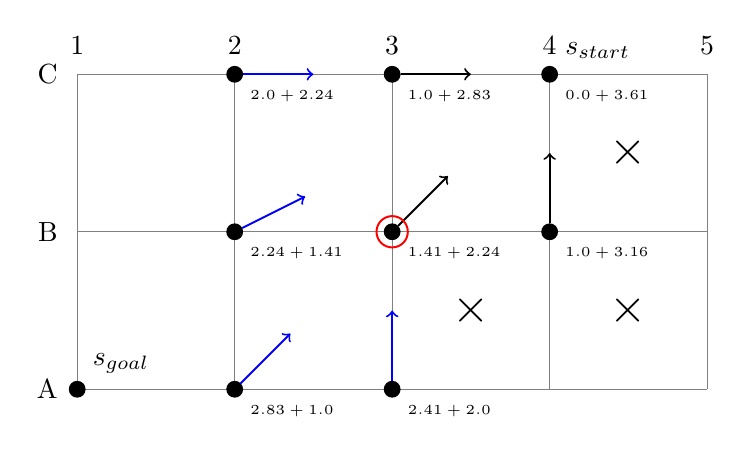
\begin{tikzpicture}[scale=2.0]
\draw [step=1.cm, color=gray] (0, 0) grid (4, 2);
\node [label=left:{C}] at (0, 2) {};
\node [label=left:{B}] at (0, 1) {};
\node [label=left:{A}] at (0, 0) {};
\node [label=above:{1}] at (0, 2) {};
\node [label=above:{2}] at (1, 2) {};
\node [label=above:{3}] at (2, 2) {};
\node [label=above:{4}] at (3, 2) {};
\node [label=above:{5}] at (4, 2) {};

\node at (3.5, 1.5) {\LARGE $\times$};
\node at (2.5, 0.5) {\LARGE $\times$};
\node at (3.5, 0.5) {\LARGE $\times$};

\node [label=above right:{$s_{start}$}, label=below right:{\tiny$0.0 + 3.61$}, draw, circle, fill, inner sep=2pt] (start) at (3, 2) {};
\node [label=above right:{$s_{goal}$}, draw, circle, fill, inner sep=2pt] at (0, 0) {};

\node [label=below right:{\tiny$1.0 + 2.83$}, draw, circle, fill, inner sep=2pt] (C3) at (2, 2) {};
\node [label=below right:{\tiny$1.41 + 2.24$}, draw, circle, fill, inner sep=2pt] (B3) at (2, 1) {};
\node [label=below right:{\tiny$1.0 + 3.16$}, draw, circle, fill, inner sep=2pt] (B4) at (3, 1) {};
\draw [->, line width=0.25mm, black] (C3) -- ($(C3)!0.5cm!(start)$);
\draw [->, line width=0.25mm, black] (B3) -- ($(B3)!0.5cm!(start)$);
\draw [->, line width=0.25mm, black] (B4) -- ($(B4)!0.5cm!(start)$);

\node [draw, circle, color=red, line width=0.25mm, inner sep=4pt] at (B3) {};

\node [label=below right:{\tiny$2.41 + 2.0$}, draw, circle, fill, inner sep=2pt] (A3) at (2, 0) {};
\node [label=below right:{\tiny$2.0 + 2.24$}, draw, circle, fill, inner sep=2pt] (C2) at (1, 2) {};
\node [label=below right:{\tiny$2.24 + 1.41$}, draw, circle, fill, inner sep=2pt] (B2) at (1, 1) {};
\node [label=below right:{\tiny$2.83 + 1.0$}, draw, circle, fill, inner sep=2pt] (A2) at (1, 0) {};
\draw [->, line width=0.25mm, blue] (A3) -- ($(A3)!0.5cm!(B3)$);
\draw [->, line width=0.25mm, blue] (C2) -- ($(C2)!0.5cm!(start)$);
\draw [->, line width=0.25mm, blue] (B2) -- ($(B2)!0.5cm!(start)$);
\draw [->, line width=0.25mm, blue] (A2) -- ($(A2)!0.5cm!(start)$);
\end{tikzpicture}

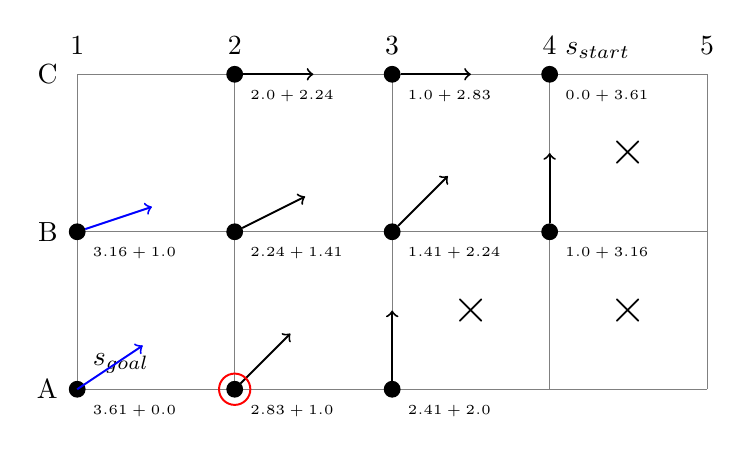
\begin{tikzpicture}[scale=2.0]
\draw [step=1.cm, color=gray] (0, 0) grid (4, 2);
\node [label=left:{C}] at (0, 2) {};
\node [label=left:{B}] at (0, 1) {};
\node [label=left:{A}] at (0, 0) {};
\node [label=above:{1}] at (0, 2) {};
\node [label=above:{2}] at (1, 2) {};
\node [label=above:{3}] at (2, 2) {};
\node [label=above:{4}] at (3, 2) {};
\node [label=above:{5}] at (4, 2) {};

\node at (3.5, 1.5) {\LARGE $\times$};
\node at (2.5, 0.5) {\LARGE $\times$};
\node at (3.5, 0.5) {\LARGE $\times$};

\node [label=above right:{$s_{start}$}, label=below right:{\tiny$0.0 + 3.61$}, draw, circle, fill, inner sep=2pt] (start) at (3, 2) {};
\node [label=above right:{$s_{goal}$}, label=below right:{\tiny$3.61 + 0.0$}, draw, circle, fill, inner sep=2pt] at (0, 0) {};

\node [label=below right:{\tiny$1.0 + 2.83$}, draw, circle, fill, inner sep=2pt] (C3) at (2, 2) {};
\node [label=below right:{\tiny$1.41 + 2.24$}, draw, circle, fill, inner sep=2pt] (B3) at (2, 1) {};
\node [label=below right:{\tiny$1.0 + 3.16$}, draw, circle, fill, inner sep=2pt] (B4) at (3, 1) {};
\draw [->, line width=0.25mm, black] (C3) -- ($(C3)!0.5cm!(start)$);
\draw [->, line width=0.25mm, black] (B3) -- ($(B3)!0.5cm!(start)$);
\draw [->, line width=0.25mm, black] (B4) -- ($(B4)!0.5cm!(start)$);

\node [label=below right:{\tiny$2.41 + 2.0$}, draw, circle, fill, inner sep=2pt] (A3) at (2, 0) {};
\node [label=below right:{\tiny$2.0 + 2.24$}, draw, circle, fill, inner sep=2pt] (C2) at (1, 2) {};
\node [label=below right:{\tiny$2.24 + 1.41$}, draw, circle, fill, inner sep=2pt] (B2) at (1, 1) {};
\node [label=below right:{\tiny$2.83 + 1.0$}, draw, circle, fill, inner sep=2pt] (A2) at (1, 0) {};
\draw [->, line width=0.25mm, black] (A3) -- ($(A3)!0.5cm!(B3)$);
\draw [->, line width=0.25mm, black] (C2) -- ($(C2)!0.5cm!(start)$);
\draw [->, line width=0.25mm, black] (B2) -- ($(B2)!0.5cm!(start)$);
\draw [->, line width=0.25mm, black] (A2) -- ($(A2)!0.5cm!(start)$);

\node [draw, circle, color=red, line width=0.25mm, inner sep=4pt] at (A2) {};

\node [label=below right:{\tiny$3.16 + 1.0$}, draw, circle, fill, inner sep=2pt] (B1) at (0, 1) {};
\draw [->, line width=0.25mm, blue] (B1) -- ($(B1)!0.5cm!(start)$);
\draw [->, line width=0.25mm, blue] (0, 0) -- ($(0, 0)!0.5cm!(start)$);
\end{tikzpicture}

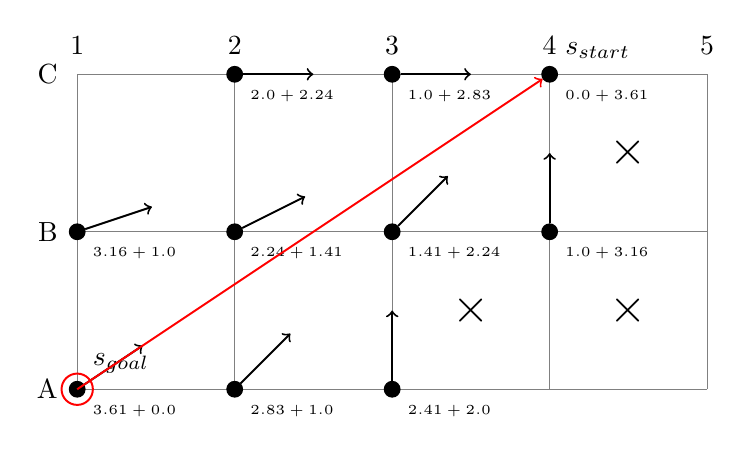
\begin{tikzpicture}[scale=2.0]
\draw [step=1.cm, color=gray] (0, 0) grid (4, 2);
\node [label=left:{C}] at (0, 2) {};
\node [label=left:{B}] at (0, 1) {};
\node [label=left:{A}] at (0, 0) {};
\node [label=above:{1}] at (0, 2) {};
\node [label=above:{2}] at (1, 2) {};
\node [label=above:{3}] at (2, 2) {};
\node [label=above:{4}] at (3, 2) {};
\node [label=above:{5}] at (4, 2) {};

\node at (3.5, 1.5) {\LARGE $\times$};
\node at (2.5, 0.5) {\LARGE $\times$};
\node at (3.5, 0.5) {\LARGE $\times$};

\node [label=above right:{$s_{start}$}, label=below right:{\tiny$0.0 + 3.61$}, draw, circle, fill, inner sep=2pt] (start) at (3, 2) {};
\node [label=above right:{$s_{goal}$}, label=below right:{\tiny$3.61 + 0.0$}, draw, circle, fill, inner sep=2pt] at (0, 0) {};

\node [label=below right:{\tiny$1.0 + 2.83$}, draw, circle, fill, inner sep=2pt] (C3) at (2, 2) {};
\node [label=below right:{\tiny$1.41 + 2.24$}, draw, circle, fill, inner sep=2pt] (B3) at (2, 1) {};
\node [label=below right:{\tiny$1.0 + 3.16$}, draw, circle, fill, inner sep=2pt] (B4) at (3, 1) {};
\draw [->, line width=0.25mm, black] (C3) -- ($(C3)!0.5cm!(start)$);
\draw [->, line width=0.25mm, black] (B3) -- ($(B3)!0.5cm!(start)$);
\draw [->, line width=0.25mm, black] (B4) -- ($(B4)!0.5cm!(start)$);

\node [label=below right:{\tiny$2.41 + 2.0$}, draw, circle, fill, inner sep=2pt] (A3) at (2, 0) {};
\node [label=below right:{\tiny$2.0 + 2.24$}, draw, circle, fill, inner sep=2pt] (C2) at (1, 2) {};
\node [label=below right:{\tiny$2.24 + 1.41$}, draw, circle, fill, inner sep=2pt] (B2) at (1, 1) {};
\node [label=below right:{\tiny$2.83 + 1.0$}, draw, circle, fill, inner sep=2pt] (A2) at (1, 0) {};
\draw [->, line width=0.25mm, black] (A3) -- ($(A3)!0.5cm!(B3)$);
\draw [->, line width=0.25mm, black] (C2) -- ($(C2)!0.5cm!(start)$);
\draw [->, line width=0.25mm, black] (B2) -- ($(B2)!0.5cm!(start)$);
\draw [->, line width=0.25mm, black] (A2) -- ($(A2)!0.5cm!(start)$);

\node [label=below right:{\tiny$3.16 + 1.0$}, draw, circle, fill, inner sep=2pt] (B1) at (0, 1) {};
\draw [->, line width=0.25mm, black] (B1) -- ($(B1)!0.5cm!(start)$);
\draw [->, line width=0.25mm, black] (0, 0) -- ($(0, 0)!0.5cm!(start)$);

\node [draw, circle, color=red, line width=0.25mm, inner sep=4pt] at (0, 0) {};

\draw [->, line width=0.25mm, red] (0,0) -- (start);
\end{tikzpicture}

\item
To implement A*, we first created a \verb|Grid| and \verb|SearchState| class.
The \verb|Grid| class is responsible for reading, writing, and storing in memory the data of a grid.
As such, it has a method that returns the unblocked neighbors of a given vertex (the $succ$ function)
as well as another method that gives the euclidean distance between two verticies (the $c$ function).
The \verb|SearchState| class is a collection of state used by A* (and later by Theta* as well).
It holds the data/implementation for the $g$ function, $parent$ function, open list, and closed list.
Using a \verb|Grid|, a \verb|SearchState|, and its own implementation of $h$,
the \verb|AStar| class is thereby able to perform the A* search algorithm.

\item
Theta* runs the same way that A* does with the difference being a small check to see
if a direct path can be made to the previous vertex's parent using the \verb|lineOfSight| function provided
in the project description. If the next vertex can still reach the older one's parent then a new shorter
direct line is made. If the old parent is not visible then the vertex is instead added the same way as
in the A* algorithm. This ensures that Theta* finds a path at least as short as A*.

\item
First, $h(s) = \sqrt{2} \cdot
  \min(|s^x - s_{goal}^x|, |s^y - s_{goal}^y|)
+ \max(|s^x - s_{goal}^x|, |s^y - s_{goal}^y|)
- \min(|s^x - s_{goal}^x|, |s^y - s_{goal}^y|)$.
The first $\min(...)$ gives us enough diagonal lines to be on either the same $x$ or $y$ (whichever is lower)
to the goal node when we move from the start node. Then, with the second half of the equation,
we get enough either vertical or horizontal lines to reach our goal.
We then get the shortest path using only $x$, $y$, and diagonal movements with no regard for blocked cells.
This is always guaranteed to find the shortest path since the values given by $h(s)$
will always either be equal to or less than the value of $g(s)$, along with all $h(n)$ and $g(n)$.
This is because $h(s)$ either is valid as the shortest path if it doesn't go through any blocked cells,
or it will be less than the shortest path if it does go through any blocked cells.
This is because if there is a blocked cell, instead of going through it with a cost of $\sqrt{2}$,
we need instead multiple 1 cost lines which will always be more than $\sqrt{2}$.
Since $h(s) \le h^*(s)$, we can conclude that it is optimistic enough to always focus on a path
where the cost is as low as it can be.

\item
Our own implementation of a binary heap stores all values in an array in level order
(with the lowest value at the top of the tree).
When an entry is added or removed, a siftdown or siftup operation is made to ensure its heap property is maintained.
Naturally, the type of element in the heap must implement \verb|Comparable|.
In the \verb|SearchState| class, the fringe is implemented as a heap
and the entry type is defined as having a vertex field, a $g$ value and a $h$ value.
The comparison between entries is made to prefer vertices with lower distance $f$ and higher $g$ in the case of a tie.
This ensures that the shortest distance is chosen, and in a tie, preferring to stay on the current path.

\item
In our original implemention, the state kept by the search algorithm ($g$, $parent$, and $closed$)
was stored using arrays. That is, the length of these arrays was (roughly) equal to the number of verticies
regardless of whether only one or all of the verticies were visited.
As such, the memory usage scaled quadratically with grid side length (assume a square grid).
Additionally, some of the arrays were being initialized to a default value (e.g., $\infty$),
and so there was also a runtime cost that scaled quadratically with grid side length.

The optimized implementation uses hashtables and hashsets to store the state for the search algorithm.
With this, only the state of the visited vertices would be stored,
and so the memory usage would scale based off of that.
This would also eliminate the need to set the initial value for every vertex.
As one can see based off of the A* and Theta* memory usage graphs below,
this drastically reduces the amount of memory used.
It also noticeably reduces the runtime for A*.
However, the runtime for Theta* became noticably slower.
To our best understanding
\footnote{Through the `jstat -gc' command we have determined that the increase
in runtime is not due to garbage collection.},
this is because Theta* expands relatively more verticies compared to A* (see h)).
As a result, this amplifies the larger overhead
\footnote{E.g., every single hashtable/hashset lookup or insert has to create a new Integer object
in order to autobox the incoming primitive int.}
to get and set values from hashtables and hashsets compared to a simple array read or write.
These additional, more costly lookups and inserts are enough to more than offset
any runtime reduction resulting from not needing to set default values.

The results for the running time and memory usage are shown below.
(Note that the $x$-axis scale is exponential.)
For these tests, the approximate distance, $d$, between the start and goal
was set to be half of the side length of the grid.
Runtimes are reported by taking the difference in the start and end miliseconds
as reported by Java's \verb|System| class.
Memory usage is reported by the command \verb|jmap -histo:live|.

\begin{filecontents}{optimize_a_time.dat}
n     Array  Hash
150     2.6    3.6
300     5.4    4.3
600     8.1    6.4
1200   16.9   10.9
2400   29.7   19.7
4800   86.1   56.5
9600  281.2  114.4
\end{filecontents}

\begin{figure}[h!]
\begin{tikzpicture}
  \begin{axis}[
    title={
      A* Runtime Averaged Over 50 Random Square Grids\\
      with 10\% Blocked Cells and $d=0.5$
    },
    title style={align=center},
    width=12cm,
    height=8cm,
    xmode=log,
    xmin=150,
    xlabel=Grid Side Length,
    xticklabels from table={optimize_a_time.dat}{n},
    xtick=data,
    ymin=0,
    ylabel=Avg. Running Time (ms),
    legend pos=north west
  ]
    \addplot[green,thick,mark=square*] table [y=Hash,x=n]{optimize_a_time.dat};
    \addlegendentry{Hash Implementation}
    \addplot[red,thick,mark=square*] table [y=Array,x=n]{optimize_a_time.dat};
    \addlegendentry{Array Implementation}
  \end{axis}
\end{tikzpicture}
\end{figure}

\begin{filecontents}{optimize_a_mem.dat}
n     Array   Hash
600      4.9   0.9
1200    17.7   1.3
2400    68.5   3.2
4800   271.0   8.5
9600  1126.4  20.0
\end{filecontents}

\begin{figure}[h!]
\begin{tikzpicture}
  \begin{axis}[
    title={
      A* Memory Usage Averaged Over 30 Random Square Grids\\
      with 10\% Blocked Cells and $d=0.5$
    },
    title style={align=center},
    width=12cm,
    height=8cm,
    xmode=log,
    xmin=600,
    xlabel=Grid Side Length,
    xticklabels from table={optimize_a_mem.dat}{n},
    xtick=data,
    ymin=0,
    ylabel=Memory Usage (MiB),
    ylabel style={yshift=10pt},
    legend pos=north west
  ]
    \addplot[green,thick,mark=square*] table [y=Hash,x=n]{optimize_a_mem.dat};
    \addlegendentry{Hash Implementation}
    \addplot[red,thick,mark=square*] table [y=Array,x=n]{optimize_a_mem.dat};
    \addlegendentry{Array Implementation}
  \end{axis}
\end{tikzpicture}
\end{figure}

\begin{filecontents}{optimize_t_time.dat}
n     Array   Hash
150     4.02     5.90
300     9.40     9.60
600    18.52    17.14
1200   33.38    43.56
2400   77.34   120.94
4800  254.24   393.24
9600  966.10  1657.08
\end{filecontents}

\begin{figure}[h!]
\begin{tikzpicture}
  \begin{axis}[
    title={
      Theta* Runtime Averaged Over 50 Random Square Grids\\
      with 10\% Blocked Cells and $d=0.5$
    },
    title style={align=center},
    width=12cm,
    height=8cm,
    xmode=log,
    xmin=150,
    xlabel=Grid Side Length,
    xticklabels from table={optimize_t_time.dat}{n},
    xtick=data,
    ymin=0,
    ylabel=Avg. Running Time (ms),
    ylabel style={yshift=10pt},
    ytick={0, 250, 500, 750, 1000, 1250, 1500, 1750},
    legend pos=north west
  ]
    \addplot[green,thick,mark=square*] table [y=Hash,x=n]{optimize_t_time.dat};
    \addlegendentry{Hash Implementation}
    \addplot[red,thick,mark=square*] table [y=Array,x=n]{optimize_t_time.dat};
    \addlegendentry{Array Implementation}
  \end{axis}
\end{tikzpicture}
\end{figure}

\begin{filecontents}{optimize_t_mem.dat}
n     Array   Hash
600      4.9   0.9
1200    17.7   1.3
2400    68.5   3.0
4800   271.1   8.4
9600  1126.4  20.0
\end{filecontents}

\begin{figure}[h!]
\begin{tikzpicture}
  \begin{axis}[
    title={
      Theta* Memory Usage Averaged Over 30 Random Square Grids\\
      with 10\% Blocked Cells and $d=0.5$
    },
    title style={align=center},
    width=12cm,
    height=8cm,
    xmode=log,
    xmin=600,
    xlabel=Grid Side Length,
    xticklabels from table={optimize_t_mem.dat}{n},
    xtick=data,
    ymin=0,
    ylabel=Memory Usage (MiB),
    ylabel style={yshift=10pt},
    legend pos=north west
  ]
    \addplot[green,thick,mark=square*] table [y=Hash,x=n]{optimize_t_mem.dat};
    \addlegendentry{Hash Implementation}
    \addplot[red,thick,mark=square*] table [y=Array,x=n]{optimize_t_mem.dat};
    \addlegendentry{Array Implementation}
  \end{axis}
\end{tikzpicture}
\end{figure}

\pagebreak

\item
Like in g), the runtimes for A* and Theta* across the same 50 grids
were gathered through Java's \verb|System| class.
In addition, the program reported the resulting path length for each grid and algorithm.
See Table \ref{table:runtime} and Table \ref{table:pathLength} in the appendix for the data gathered.
Looking at the resulting path lengths for each grid,
the path length from A* is always greater than or equal to the path length from Theta*.
To help illustrate this, A* gave a average path length of 45.5667 across the 50 grids,
which is higher than Theta*'s average path length of 43.2994.
As mentioned in d), this can be explained by the fact that Theta* considers not only the path considered by A*
but also another potentially shorter path from the parent of the vertex.
That is, A*'s path lengths can only be greater than or equal to the path lengths given by Theta* (for the same grid).

On the other hand, Theta* appears to be more computationally expensive than A*.
The average runtime of Theta* accross the 50 grids is 3.06ms,
which is higher than A*'s average runtime of 1.74ms.
In fact, Theta* took less time than A* in only 1 of the 50 grids.
This could be because Theta* not only has to check for line of sight,
but also because it tends to expand more vertices.
This can been seen from Table \ref{table:closed} in the appendix
which provides the number of closed verticies over the 50 grids.
Theta*'s average was 124.72 vertices,
which is almost 3 times A*'s average of 43.98.
So, at least for these kinds of grids,
Theta* will tend to have a longer runtime than A*.

The runtimes above were gathered using our own binary heap implementation as described in f).
Table \ref{table:runtime-pq} in the appendix gives the runtimes when using the standard Java \verb|PriorityQueue|.
Compared to our A* and Theta* average runtimes of 1.74ms and 3.06ms respectively,
using the Java \verb|PriorityQueue| gave higher average runtimes of 2.12ms and 3.70ms.
Experiments with larger grid sizes yielded the same pattern,
so it can be concluded that our binary heap implementation improved the runtime
\footnote{Then again, benchmarking can be tricky given the quirks of modern hardware.
See \href{https://youtu.be/r-TLSBdHe1A?t=687}{``Performance Matters'' by Emery Berger} if interested.}.

\item
It is appropriate for A* and Theta* to use different h-values,
since they construct paths with different properties.
In a path generated by A*, each vertex must be a neighbor of the previous vertex in the path.
As such, an A* path consists of segments of only length 1 or $\sqrt{2}$.
It is therefore necessary to to express the h-values for A* in terms of
some number of length $\sqrt{2}$ segments and some number of length $1$ segments.
Theta*, on the other hand, constructs an any-angle path and is not limited to segments of fixed length.
I.e., the parent of a vertex in the path need not be one of its neighbors.
Because any angle / parent vertex is allowed (provided there is line of sight),
then the minimal possible distance (the eculidian distance) to the goal may be possible.
So, using this for the h-values in Theta* is appropriate.

\item
Test grids 1, 12, 14, 21, 29, 30, 41, 46 and 47 had minimal paths shorter than what was found by Theta*.

\begin{tabular}{|l|r|r|r|}
\hline
Grid & A* & Theta* & Minimal \\
\hline
1  & 33.899 & 32.083 & 32.071 \\
12 & 96.598 & 89.888 & 89.837 \\
14 & 54.971 & 51.734 & 51.673 \\
21 & 42.941 & 41.075 & 40.938 \\
29 & 70.314 & 67.844 & 67.708 \\
30 & 56.314 & 53.911 & 53.891 \\
41 & 15.243 & 14.487 & 14.369 \\
46 & 53.385 & 50.073 & 50.070 \\
47 & 79.882 & 77.168 & 77.114 \\
\hline
\end{tabular}

\item (Not attempted.)

\item Theta* expands $B2$ before $B3$ and $f(B2) = 4.576 \ge f(B3) = 4.472$.

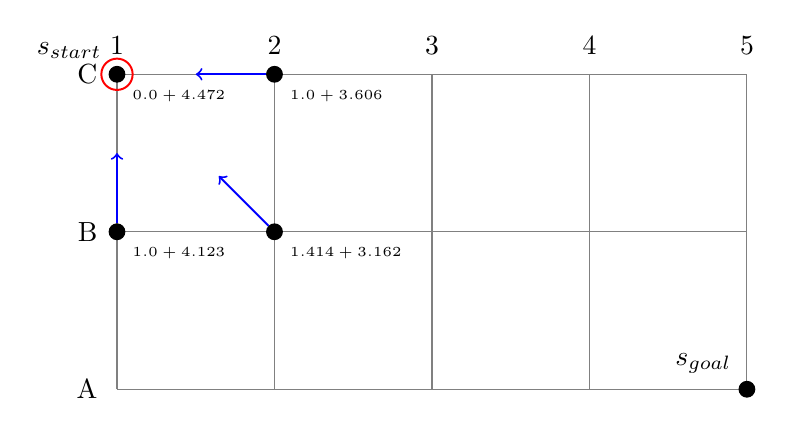
\begin{tikzpicture}[scale=2.0]
\draw [step=1.cm, color=gray] (0, 0) grid (4, 2);
\node [label=left:{C}] at (0, 2) {};
\node [label=left:{B}] at (0, 1) {};
\node [label=left:{A}] at (0, 0) {};
\node [label=above:{1}] at (0, 2) {};
\node [label=above:{2}] at (1, 2) {};
\node [label=above:{3}] at (2, 2) {};
\node [label=above:{4}] at (3, 2) {};
\node [label=above:{5}] at (4, 2) {};

\node [label=above left:{$s_{start}$}, label=below right:{\tiny$0.0 + 4.472$}, draw, circle, fill, inner sep=2pt] (start) at (0, 2) {};
\node [label=above left:{$s_{goal}$}, draw, circle, fill, inner sep=2pt] at (4, 0) {};

\node [draw, circle, color=red, line width=0.25mm, inner sep=4pt] at (start) {};

\node [label=below right:{\tiny$1.414 + 3.162$}, draw, circle, fill, inner sep=2pt] (B2) at (1, 1) {};
\node [label=below right:{\tiny$1.0 + 3.606$}, draw, circle, fill, inner sep=2pt] (C2) at (1, 2) {};
\node [label=below right:{\tiny$1.0 + 4.123$}, draw, circle, fill, inner sep=2pt] (B1) at (0, 1) {};
\draw [->, line width=0.25mm, blue] (B2) -- ($(B2)!0.5cm!(start)$);
\draw [->, line width=0.25mm, blue] (C2) -- ($(C2)!0.5cm!(start)$);
\draw [->, line width=0.25mm, blue] (B1) -- ($(B1)!0.5cm!(start)$);
\end{tikzpicture}

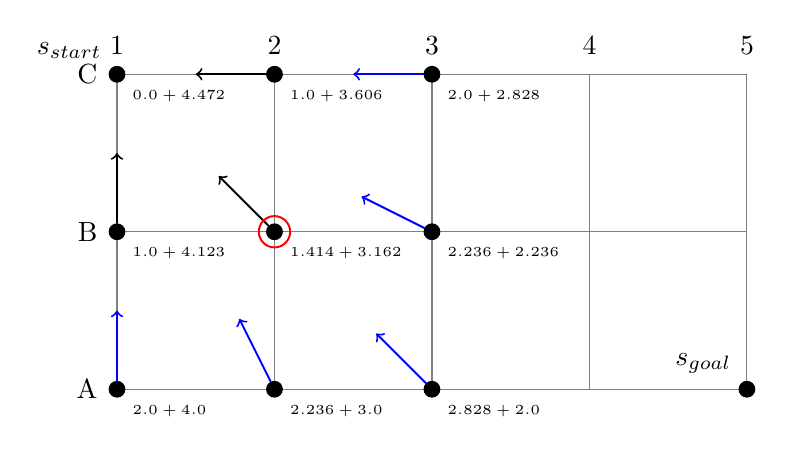
\begin{tikzpicture}[scale=2.0]
\draw [step=1.cm, color=gray] (0, 0) grid (4, 2);
\node [label=left:{C}] at (0, 2) {};
\node [label=left:{B}] at (0, 1) {};
\node [label=left:{A}] at (0, 0) {};
\node [label=above:{1}] at (0, 2) {};
\node [label=above:{2}] at (1, 2) {};
\node [label=above:{3}] at (2, 2) {};
\node [label=above:{4}] at (3, 2) {};
\node [label=above:{5}] at (4, 2) {};

\node [label=above left:{$s_{start}$}, label=below right:{\tiny$0.0 + 4.472$}, draw, circle, fill, inner sep=2pt] (start) at (0, 2) {};
\node [label=above left:{$s_{goal}$}, draw, circle, fill, inner sep=2pt] at (4, 0) {};

\node [label=below right:{\tiny$1.414 + 3.162$}, draw, circle, fill, inner sep=2pt] (B2) at (1, 1) {};
\node [label=below right:{\tiny$1.0 + 3.606$}, draw, circle, fill, inner sep=2pt] (C2) at (1, 2) {};
\node [label=below right:{\tiny$1.0 + 4.123$}, draw, circle, fill, inner sep=2pt] (B1) at (0, 1) {};
\draw [->, line width=0.25mm, black] (B2) -- ($(B2)!0.5cm!(start)$);
\draw [->, line width=0.25mm, black] (C2) -- ($(C2)!0.5cm!(start)$);
\draw [->, line width=0.25mm, black] (B1) -- ($(B1)!0.5cm!(start)$);

\node [draw, circle, color=red, line width=0.25mm, inner sep=4pt] at (B2) {};

\node [label=below right:{\tiny$2.0 + 2.828$}, draw, circle, fill, inner sep=2pt] (C3) at (2, 2) {};
\node [label=below right:{\tiny$2.236 + 2.236$}, draw, circle, fill, inner sep=2pt] (B3) at (2, 1) {};
\node [label=below right:{\tiny$2.828 + 2.0$}, draw, circle, fill, inner sep=2pt] (A3) at (2, 0) {};
\node [label=below right:{\tiny$2.236 + 3.0$}, draw, circle, fill, inner sep=2pt] (A2) at (1, 0) {};
\node [label=below right:{\tiny$2.0 + 4.0$}, draw, circle, fill, inner sep=2pt] (A1) at (0, 0) {};
\draw [->, line width=0.25mm, blue] (C3) -- ($(C3)!0.5cm!(start)$);
\draw [->, line width=0.25mm, blue] (B3) -- ($(B3)!0.5cm!(start)$);
\draw [->, line width=0.25mm, blue] (A3) -- ($(A3)!0.5cm!(start)$);
\draw [->, line width=0.25mm, blue] (A2) -- ($(A2)!0.5cm!(start)$);
\draw [->, line width=0.25mm, blue] (A1) -- ($(A1)!0.5cm!(start)$);
\end{tikzpicture}

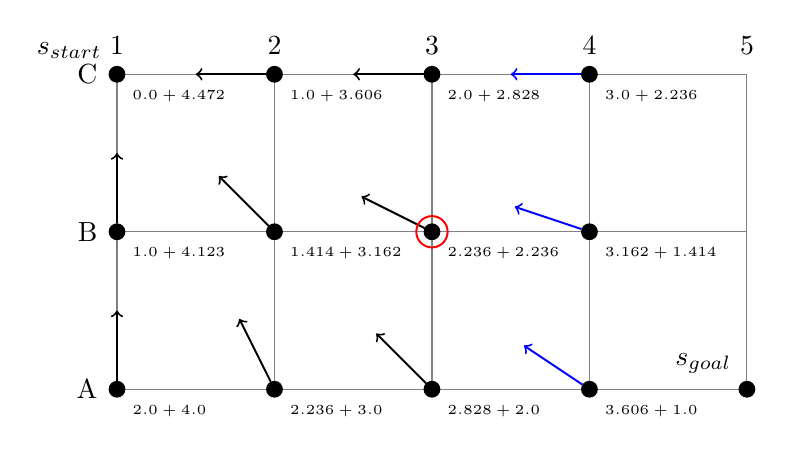
\begin{tikzpicture}[scale=2.0]
\draw [step=1.cm, color=gray] (0, 0) grid (4, 2);
\node [label=left:{C}] at (0, 2) {};
\node [label=left:{B}] at (0, 1) {};
\node [label=left:{A}] at (0, 0) {};
\node [label=above:{1}] at (0, 2) {};
\node [label=above:{2}] at (1, 2) {};
\node [label=above:{3}] at (2, 2) {};
\node [label=above:{4}] at (3, 2) {};
\node [label=above:{5}] at (4, 2) {};

\node [label=above left:{$s_{start}$}, label=below right:{\tiny$0.0 + 4.472$}, draw, circle, fill, inner sep=2pt] (start) at (0, 2) {};
\node [label=above left:{$s_{goal}$}, draw, circle, fill, inner sep=2pt] at (4, 0) {};

\node [label=below right:{\tiny$1.414 + 3.162$}, draw, circle, fill, inner sep=2pt] (B2) at (1, 1) {};
\node [label=below right:{\tiny$1.0 + 3.606$}, draw, circle, fill, inner sep=2pt] (C2) at (1, 2) {};
\node [label=below right:{\tiny$1.0 + 4.123$}, draw, circle, fill, inner sep=2pt] (B1) at (0, 1) {};
\draw [->, line width=0.25mm, black] (B2) -- ($(B2)!0.5cm!(start)$);
\draw [->, line width=0.25mm, black] (C2) -- ($(C2)!0.5cm!(start)$);
\draw [->, line width=0.25mm, black] (B1) -- ($(B1)!0.5cm!(start)$);

\node [label=below right:{\tiny$2.0 + 2.828$}, draw, circle, fill, inner sep=2pt] (C3) at (2, 2) {};
\node [label=below right:{\tiny$2.236 + 2.236$}, draw, circle, fill, inner sep=2pt] (B3) at (2, 1) {};
\node [label=below right:{\tiny$2.828 + 2.0$}, draw, circle, fill, inner sep=2pt] (A3) at (2, 0) {};
\node [label=below right:{\tiny$2.236 + 3.0$}, draw, circle, fill, inner sep=2pt] (A2) at (1, 0) {};
\node [label=below right:{\tiny$2.0 + 4.0$}, draw, circle, fill, inner sep=2pt] (A1) at (0, 0) {};
\draw [->, line width=0.25mm, black] (C3) -- ($(C3)!0.5cm!(start)$);
\draw [->, line width=0.25mm, black] (B3) -- ($(B3)!0.5cm!(start)$);
\draw [->, line width=0.25mm, black] (A3) -- ($(A3)!0.5cm!(start)$);
\draw [->, line width=0.25mm, black] (A2) -- ($(A2)!0.5cm!(start)$);
\draw [->, line width=0.25mm, black] (A1) -- ($(A1)!0.5cm!(start)$);

\node [draw, circle, color=red, line width=0.25mm, inner sep=4pt] at (B3) {};

\node [label=below right:{\tiny$3.0 + 2.236$}, draw, circle, fill, inner sep=2pt] (C4) at (3, 2) {};
\node [label=below right:{\tiny$3.162 + 1.414$}, draw, circle, fill, inner sep=2pt] (B4) at (3, 1) {};
\node [label=below right:{\tiny$3.606 + 1.0$}, draw, circle, fill, inner sep=2pt] (A4) at (3, 0) {};
\draw [->, line width=0.25mm, blue] (C4) -- ($(C4)!0.5cm!(start)$);
\draw [->, line width=0.25mm, blue] (B4) -- ($(B4)!0.5cm!(start)$);
\draw [->, line width=0.25mm, blue] (A4) -- ($(A4)!0.5cm!(start)$);
\end{tikzpicture}

The h-values for $B2$ and $B3$ are consistent, since:
\begin{align*}
h(B3) = 2.236 \le c(B3, B2) + h(B3) = 1.0 + 3.162 = 4.162 \\
h(B2) = 3.162 \le c(B2, B3) + h(B2) = 1.0 + 2.236 = 3.236
\end{align*}
This same process can be be used to show all h-values are consistent.

This makes sense, because both $c$ and $h$ are based off of the distance formula.
That is, $n$, $n'$, and $s_{goal}$ must form a triangle (or line) if there are no blocked cells.
Because $h(n)$, $c(n, n')$, and $h(n')$ each correspond to separate legs of this triangle,
then triangle inequality can be used to show that all the above h-values must be consistent.

\end{enumerate}

\section{}
\begin{enumerate}[label={\large\textbf{\alph*)}}]
\item
\Tree [.(1,4) [.(2,4) [.(2,3) [.(1,3) [.(1,2) [.(3,2) [.(3,4) \qroof{?}.\boxed{\boxed{(2,4)}} ] \qroof{-1}.\boxed{(3,1)} ] ] \qroof{?}.\boxed{\boxed{(1,4)}} ] \qroof{+1}.\boxed{(4,3)} ] ] ]

\Tree [.(1,4) [.(2,4) [.(2,3) [.(1,3) [.(1,2) [.(3,2) [.(3,4) \qroof{+1}.\boxed{\boxed{(2,4)}} ] \qroof{-1}.\boxed{(3,1)} ] ] \qroof{+1}.\boxed{\boxed{(1,4)}} ] \qroof{+1}.\boxed{(4,3)} ] ] ]

\item
Both states that result in a loop were given the value +1,
because if the agent makes the second decision instead of the loop, victory is forced for player A.

\item
One problem that can occur with minimax is that the default nodes it checks
could lead to a potential loop where is cannot reach a terminal state.
In order to avoid this problem, a list of which states have been visited before can be kept,
and if a state is revisted causing a loop then its child that has also been visited should skipped
and then another child should be checked.

\item
Each player must make $M$ moves to reach the opposite end of the array to win.
If an agent moves opposite the direction of the objective so much as once, the path length increases to $M + 2$
for that respective player, since they must move again to return to the initial position.
Even if that player hops over the other it will save one move and $M < M + 1$,
so the one player who doesn't go backwards always wins.
Now in the case of an even sized array, each player will move $M/2$ times before meeting in the middle,
and since A went first, agent B will make move $M/2$ second,
thus allowing agent A to hop over and decrease their path length to $M-1$, which ensures A's victory.
In the case of an odd sized array, each player will move $(M-1)/2$ times
and this time there will be one spot in between them. A will move first into the middle spot
which allows B to hop and have a shorter path.
Despite A being first, on A's $M-1$ move B will reach its destination thus winning the game.
Therefore, A always wins in the even case and B always in the odd case.
\end{enumerate}

\section{}
\begin{enumerate}[label={\large\textbf{\alph*)}}]
\item Hill climbing works better than simulated annealing for problems where there is no local maxima/minima, since hill climbing will \textbf{always} go for the optimal value increase in comparison to simulated annealing, which can sometimes go for suboptimal solutions on the way to the top, and may even have a chance to go over it assuming it's not the absolute maximum/minimum.
\pagebreak
\item Random guessing works just as well as simulated annealing when there isn't really a cost that we have as we move, meaning that simulated annealing's probability check becomes $1/p$, $p$ being just the number of possible choices. This is then pretty much equivalent to just randomly choosing, which has a chance of getting a spot with $1/c$, $c$ being the possible choices and is just the same as simulated with just a larger pool of choices.
\item The best problems for simulated annealing are problems that have an absolute maximum/minimum, a couple of local maxima/minima, as well as possible plateaus. This means that the function is generally not fully flat or a single maximum/minimum.
\item If simulated annealing stops at the current state that we reach when temperature and schedule reach a certain point, yet we know the goodness of each state we've checked, then just see which of the states we've visited, including the current, has the highest goodness.
\item If we have access to 2 million states instead of just 2, we could simply do ``simulated annealing'' in all directions, and possible with multiple starting spots as well. This means that we can get the value of simulated annealing (choosing suboptimal but overall positive moves) without needing to use probability to decide the next state. We can also remember states, meaning if certain paths are suboptimal overall, we can free that memory and check for any other paths that memory can be used for.
\end{enumerate}

\section{}
\begin{enumerate}[label={\large\textbf{\alph*)}}]
\item Sudoku as a constraint satisfaction problem can be represented as:
\begin{itemize}
\item Variables: $C_{i, j}$: where $i, j = 1, 2, \dots, 8, 9$ and $C$ represents a cell in the sudoku board
\item Domain: numbers from 1-9
\item Constraint: Each row and column should not have duplicates, and each $3 \times 3$ grid where $i$, $j$ are either 1-3, 4-6, or 7-9 should not have duplicates
\end{itemize}

\item Sudoku as an incremental formulation problem:
\begin{itemize}
\item Start state: state where we have filled in all the cells that are pre-done on the board, and everything else remains empty
\item Successor function: we add a number that fits within the constraints present at the time, and fill in starting from the top left, going right until the end before returning to the left and going down 1 row.
\item Goal test: is every variable filled, and does the board itself satisfy the constraints of no row, column, and $3 \times 3$ cube having a duplicate?
\item There really isn't a cost in the formula itself, so the cost can either be 0 in general or 1 just for keeping track of moves.
\item In regards with Sudoku as an incremental formulation problem, it's best to go for a remaining values heuristic, since even if you choose an ``optimal'' value, that also means that backtracking will be more frequent. It's better to go for remaining values since there's less of a chance to have to excessively backtrack.
\item Branching factor: 9, since there's 9 different choices
\item The solution depth is 81 (the size of the empty board) minus the number of variables we have
\item The max depth is 81, since it's the total number of choices we can have ever
\item The state space is $9^{\text{solution depth}}$, since we at worst go to the depth of the solution depth and have to expand each node at worst 9.
\end{itemize}
\item The difference between easy and hard sudoku puzzles is basically either better number placement or more numbers. More numbers means the solution depth is lowered meaning less possible states to go through, and better number placement reduces the times we need to go with a higher branching factor, as better number placement allows for more certainties when choosing numbers.
\pagebreak
\item Pseudocode for local search Sudoku:
\begin{verbatim}
let cells = some input sudoku board
let temperature = initial temperature
let assigned = empty set

for cell in cells:
  if cell has a number:
    add cell to assigned
  else:
    put a random number into cell

for cells not in assigned:
  calculate and store the number of
  violations for the cell

while solution not found:
  let cell = random cell not in assigned

  for n in 1 to 9:
    calculate the change in number of violations
    if cell is changed to n

  assign each n in 1 to 9 a probability based upon
  its resulting change in number of violations

  choose a random n based upon
  these probailities and temperature

  set cell to n and
  update the number of violations

  reduce(temperature)
\end{verbatim}
\end{enumerate}

\pagebreak
\section{}
Arguments:
\begin{itemize}
\item Superman's defeat: $D$
\item Kryptonite: $K$
\item Superman alone: $A$
\item Lex Luthor assist: $L$
\end{itemize}

\begin{enumerate}[label={\large\textbf{\alph*)}}]
\item $((A \land K) \Rightarrow D) \land (K \Rightarrow L) \land (L \Rightarrow \neg A)$

\item
$(\neg(A \land K) \lor D) \land (\neg K \lor L) \land (\neg L \lor \neg A) \\
= (\neg A \lor \neg K \lor D) \land (\neg K \lor L) \land (\neg L \lor \neg A)$


\item
So if we want to prove that the argument entails Superman's defeat,
we need to check if adding \textbf{not} defeating superman can be added.
\begin{align*}
& (\neg A \lor \neg K \lor D) \land (\neg K \lor L) \land (\neg L \lor \neg A) \land \neg D \\
& =(\neg A \lor \neg K \lor D) \land (\neg K) \land (\neg A) \land \neg D \\
&= (\neg A \lor \neg K) \land (\neg K) \land (\neg A)
\end{align*}

We're left with only the parts that prevent us from defeating Superman, meaning it's still $\neg D$.
\end{enumerate}

\pagebreak

\renewcommand\thesection{}
\renewcommand\thesubsection{}
\section{\underline{Appendix}}

\begin{longtable}{|l|r|r|}
\caption{A* and Theta* Runtimes (in ms) for 50 Grids}
\label{table:runtime} \\
\hline
Grid & A* & Theta* \\
\hline
1  & 2 & 3 \\
2  & 2 & 4 \\
3  & 2 & 3 \\
4  & 1 & 2 \\
5  & 2 & 3 \\
6  & 2 & 2 \\
7  & 2 & 4 \\
8  & 1 & 1 \\
9  & 2 & 3 \\
10 & 2 & 3 \\
11 & 2 & 5 \\
12 & 2 & 7 \\
13 & 1 & 2 \\
14 & 2 & 4 \\
15 & 1 & 3 \\
16 & 2 & 4 \\
17 & 2 & 3 \\
18 & 1 & 2 \\
19 & 1 & 2 \\
20 & 2 & 3 \\
21 & 2 & 3 \\
22 & 2 & 4 \\
23 & 1 & 1 \\
24 & 1 & 4 \\
25 & 2 & 4 \\
26 & 2 & 4 \\
27 & 2 & 3 \\
28 & 1 & 2 \\
29 & 2 & 4 \\
30 & 2 & 4 \\
31 & 1 & 2 \\
32 & 3 & 2 \\
33 & 2 & 2 \\
34 & 1 & 2 \\
35 & 2 & 1 \\
36 & 1 & 2 \\
37 & 2 & 5 \\
38 & 2 & 3 \\
39 & 1 & 3 \\
40 & 2 & 3 \\
41 & 1 & 2 \\
42 & 2 & 5 \\
43 & 2 & 3 \\
44 & 2 & 2 \\
45 & 2 & 2 \\
46 & 2 & 3 \\
47 & 2 & 6 \\
48 & 2 & 4 \\
49 & 2 & 3 \\
50 & 2 & 2 \\
\hline
Average & 1.74 & 3.06 \\
\hline
\end{longtable}

\pagebreak

\begin{longtable}{|l|r|r|}
\caption{A* and Theta* Path Length for 50 Grids}
\label{table:pathLength} \\
\hline
Grid & A* & Theta* \\
\hline
1  &  33.8990 & 32.0830 \\
2  &  86.3140 & 83.3990 \\
3  &  27.5560 & 25.5230 \\
4  &  29.0420 & 27.9390 \\
5  &  41.8990 & 39.8620 \\
6  &  26.6270 & 25.9140 \\
7  &  62.7990 & 58.9480 \\
8  &   3.0000 &  3.0000 \\
9  &  36.1130 & 34.9870 \\
10 &  51.3850 & 48.0160 \\
11 &  59.8410 & 56.7500 \\
12 &  96.5980 & 89.8880 \\
13 &  23.3140 & 21.6970 \\
14 &  54.9710 & 51.7340 \\
15 &  51.6270 & 47.9070 \\
16 &  67.3970 & 65.5320 \\
17 &  55.8990 & 53.7390 \\
18 &  13.3140 & 12.8060 \\
19 &  12.0000 & 12.0000 \\
20 &  61.6570 & 60.2170 \\
21 &  42.9410 & 41.0750 \\
22 &  37.4140 & 37.2360 \\
23 &   9.8280 &  9.2200 \\
24 &  64.9710 & 61.3790 \\
25 &  78.6570 & 77.2840 \\
26 &  54.2130 & 50.6630 \\
27 &  35.5270 & 35.0700 \\
28 &  13.8280 & 13.3190 \\
29 &  70.3140 & 67.8440 \\
30 &  56.3140 & 53.9110 \\
31 &  26.2430 & 25.3890 \\
32 &  47.2130 & 43.7890 \\
33 &   2.0000 &  2.0000 \\
34 &  34.7990 & 32.3490 \\
35 &   4.0000 &  4.0000 \\
36 &  45.5980 & 44.1290 \\
37 & 101.0120 & 93.8660 \\
38 &  47.1420 & 44.4340 \\
39 &  41.9410 & 40.2450 \\
40 &  52.6980 & 48.7970 \\
41 &  15.2430 & 14.4870 \\
42 &  82.1130 & 76.6240 \\
43 &  44.1840 & 42.7510 \\
44 &  42.7280 & 40.1930 \\
45 &  40.9710 & 38.0610 \\
46 &  53.3850 & 50.0730 \\
47 &  79.8820 & 77.1680 \\
48 &  94.9120 & 88.1620 \\
49 &  33.9710 & 31.4660 \\
50 &  29.0420 & 28.0430 \\
\hline
Average & 45.5667 & 43.2994 \\
\hline
\end{longtable}

\pagebreak

\begin{longtable}{|l|r|r|}
\caption{A* and Theta* Number of Closed Verticies for 50 Grids}
\label{table:closed} \\
\hline
Grid & A* & Theta* \\
\hline
 1 &  31 &  91 \\
 2 &  83 & 211 \\
 3 &  23 &  43 \\
 4 &  23 &  53 \\
 5 &  39 & 104 \\
 6 &  25 &  68 \\
 7 &  69 & 195 \\
 8 &   3 &   3 \\
 9 &  27 &  69 \\
10 &  46 & 115 \\
11 &  47 & 241 \\
12 &  85 & 429 \\
13 &  20 &  52 \\
14 &  50 & 190 \\
15 &  45 & 110 \\
16 &  50 & 111 \\
17 &  69 & 185 \\
18 &  10 &  10 \\
19 &  12 &  12 \\
20 &  60 & 105 \\
21 &  33 & 106 \\
22 &  68 & 143 \\
23 &   9 &  11 \\
24 &  60 & 185 \\
25 &  77 & 241 \\
26 &  48 & 145 \\
27 &  63 & 105 \\
28 &  13 &  18 \\
29 &  67 & 331 \\
30 &  94 & 188 \\
31 &  25 &  56 \\
32 &  42 &  80 \\
33 &   2 &   2 \\
34 &  30 &  57 \\
35 &   4 &   4 \\
36 &  35 &  47 \\
37 &  89 & 366 \\
38 &  58 & 123 \\
39 &  32 &  82 \\
40 &  45 &  81 \\
41 &  14 &  26 \\
42 &  73 & 397 \\
43 &  34 &  72 \\
44 &  39 &  69 \\
45 &  36 &  49 \\
46 &  48 & 176 \\
47 &  61 & 283 \\
48 & 112 & 282 \\
49 &  29 &  43 \\
50 &  42 &  71 \\
\hline
Average & 43.98 & 124.72 \\
\hline
\end{longtable}

\pagebreak
\begin{longtable}{|l|r|r|}
\caption{A* and Theta* Runtimes (in ms) for 50 Grids using standard Java PriorityQueue}
\label{table:runtime-pq} \\
\hline
Grid & A* & Theta* \\
\hline
1  & 2 & 3 \\
2  & 3 & 4 \\
3  & 2 & 2 \\
4  & 2 & 3 \\
5  & 2 & 4 \\
6  & 2 & 3 \\
7  & 3 & 4 \\
8  & 2 & 1 \\
9  & 2 & 3 \\
10 & 2 & 3 \\
11 & 2 & 5 \\
12 & 2 & 6 \\
13 & 2 & 4 \\
14 & 2 & 5 \\
15 & 3 & 3 \\
16 & 2 & 5 \\
17 & 3 & 6 \\
18 & 1 & 2 \\
19 & 2 & 2 \\
20 & 2 & 6 \\
21 & 2 & 4 \\
22 & 2 & 4 \\
23 & 1 & 1 \\
24 & 3 & 5 \\
25 & 3 & 5 \\
26 & 2 & 4 \\
27 & 3 & 3 \\
28 & 1 & 1 \\
29 & 2 & 6 \\
30 & 3 & 4 \\
31 & 1 & 3 \\
32 & 3 & 3 \\
33 & 1 & 1 \\
34 & 2 & 3 \\
35 & 1 & 1 \\
36 & 2 & 3 \\
37 & 3 & 6 \\
38 & 3 & 3 \\
39 & 2 & 4 \\
40 & 3 & 6 \\
41 & 1 & 3 \\
42 & 2 & 6 \\
43 & 2 & 3 \\
44 & 2 & 3 \\
45 & 1 & 3 \\
46 & 2 & 5 \\
47 & 3 & 7 \\
48 & 3 & 6 \\
49 & 2 & 2 \\
50 & 2 & 3 \\
\hline
Average & 2.12 & 3.70 \\
\hline
\end{longtable}

\end{document}
